\section{Results}

\subsection{Variation in thrombolysis use}

Thrombolysis use in the original data varied between hospitals from 1.5\% to 24.3\% of all patients, and 7.3\% to 49.7\% of patients arriving within 4 hours of known stroke onset.

%%%%%%%%%%%%%%%%%%%%%%%%%%%%%%%%%%%%%%%%%%%%%%%%%%%%%%%%%%%%%%%%%%%%%%%%

\subsection{Feature selection}

In order to provide a more explainable machine learning model, the number of features were restricted to those that provide most information regarding use of thrombolysis. 25 features were selected by identifying one feature at a time that led to greatest improvement in Receiver Operating Characteristic (ROC) Area Under Curve (AUC). ROC AUC was measured using stratified 5-fold cross validation.

The best model with 1, 2, 5, 10, 25 \& all features (60 features before one-hot encoding of fields) had ROC AUCs of 0.715, 0.792, 0.891, 0.919, 0.923 \& 0.922. We selected 10 features for all subsequent work, which were:

\begin{itemize}
    \item \emph{Arrival-to-scan time}: Time from arrival at hospital to scan (mins)
    \item \emph{Infarction}: Stroke type (1 = infarction, 0 = haemorrhage)
    \item \emph{Stroke severity}: Stroke severity (NIHSS) on arrival
    \item \emph{Precise onset time}: Onset time type (1 = precise, 0 = best estimate)
    \item \emph{Prior disability level}: Disability level (modified Rankin Scale) before stroke
    \item \emph{Stroke team}: Stroke team attended
    \item \emph{Use of AF anticoagulants}: Use of atrial fibrillation anticoagulant (1 = Yes, 0 = No)
    \item \emph{Onset-to-arrival time}: Time from onset of stroke to arrival at hospital (mins)
    \item \emph{Onset during sleep}: Did stroke occur in sleep?
    \item \emph{Age}: Age (as middle of 5 year age bands)
\end{itemize}

Correlations between the 10 features were measured using coefficients of determination (r-squared). All r-squared were less than 0.15, and all r-squared were less than 0.05 except 1) age and prior disability level (r-squared 0.146), and 2) onset during sleep and precise onset time (r-squared 0.078).

%%%%%%%%%%%%%%%%%%%%%%%%%%%%%%%%%%%%%%%%%%%%%%%%%%%%%%%%%%%%%%%%%%%%%%%%

\subsection{Model accuracy}

Model accuracy was measured using stratified 5-fold cross validation. Overall accuracy was 85.0\% (83.9\% sensitivity and specificity could be achieved simultaneously). The ROC AUC was 0.918. The model predicted hospital thrombolysis use at each hospital with very good accuracy (r-squared = 0.977).

The appendix contains further accuracy measures, and results for model validation of hospital thrombolysis curves, evaluation of variation in model prediction using bagging, learning rates, model calibration, and fine-tuning of model regularisation.

%%%%%%%%%%%%%%%%%%%%%%%%%%%%%%%%%%%%%%%%%%%%%%%%%%%%%%%%%%%%%%%%%%%%%%%%

\subsection{An analysis of the characteristics of the most thrombolysable patient at each hospital}

We identified the patient with the highest probability of receiving thrombolysis (taken from 5-fold combined test set results) at each hospital, and compared the feature values of those patients to:

\begin{itemize}
    \item All patients
    \item All patients who had received thrombolysis
    \item All patients who had not received thrombolysis
\end{itemize}

As seen in figure \ref{fig:results_most_thrombolysable}, Compared with the other groups, the most thrombolysable patients 1) Had shorter arrrival-to-scan times, 2) Had an infarction stroke type, 3) Had stroke severity with NIHR 5-25, 4) Had a precise onset time, 5) Had lower pre-stroke disability, 6) Were not taking anticoagulant medication, 7) Had shorter onset-to-arrival times, 8) Did not have onset during sleep, 9) Were younger.

\begin{figure}
\centering
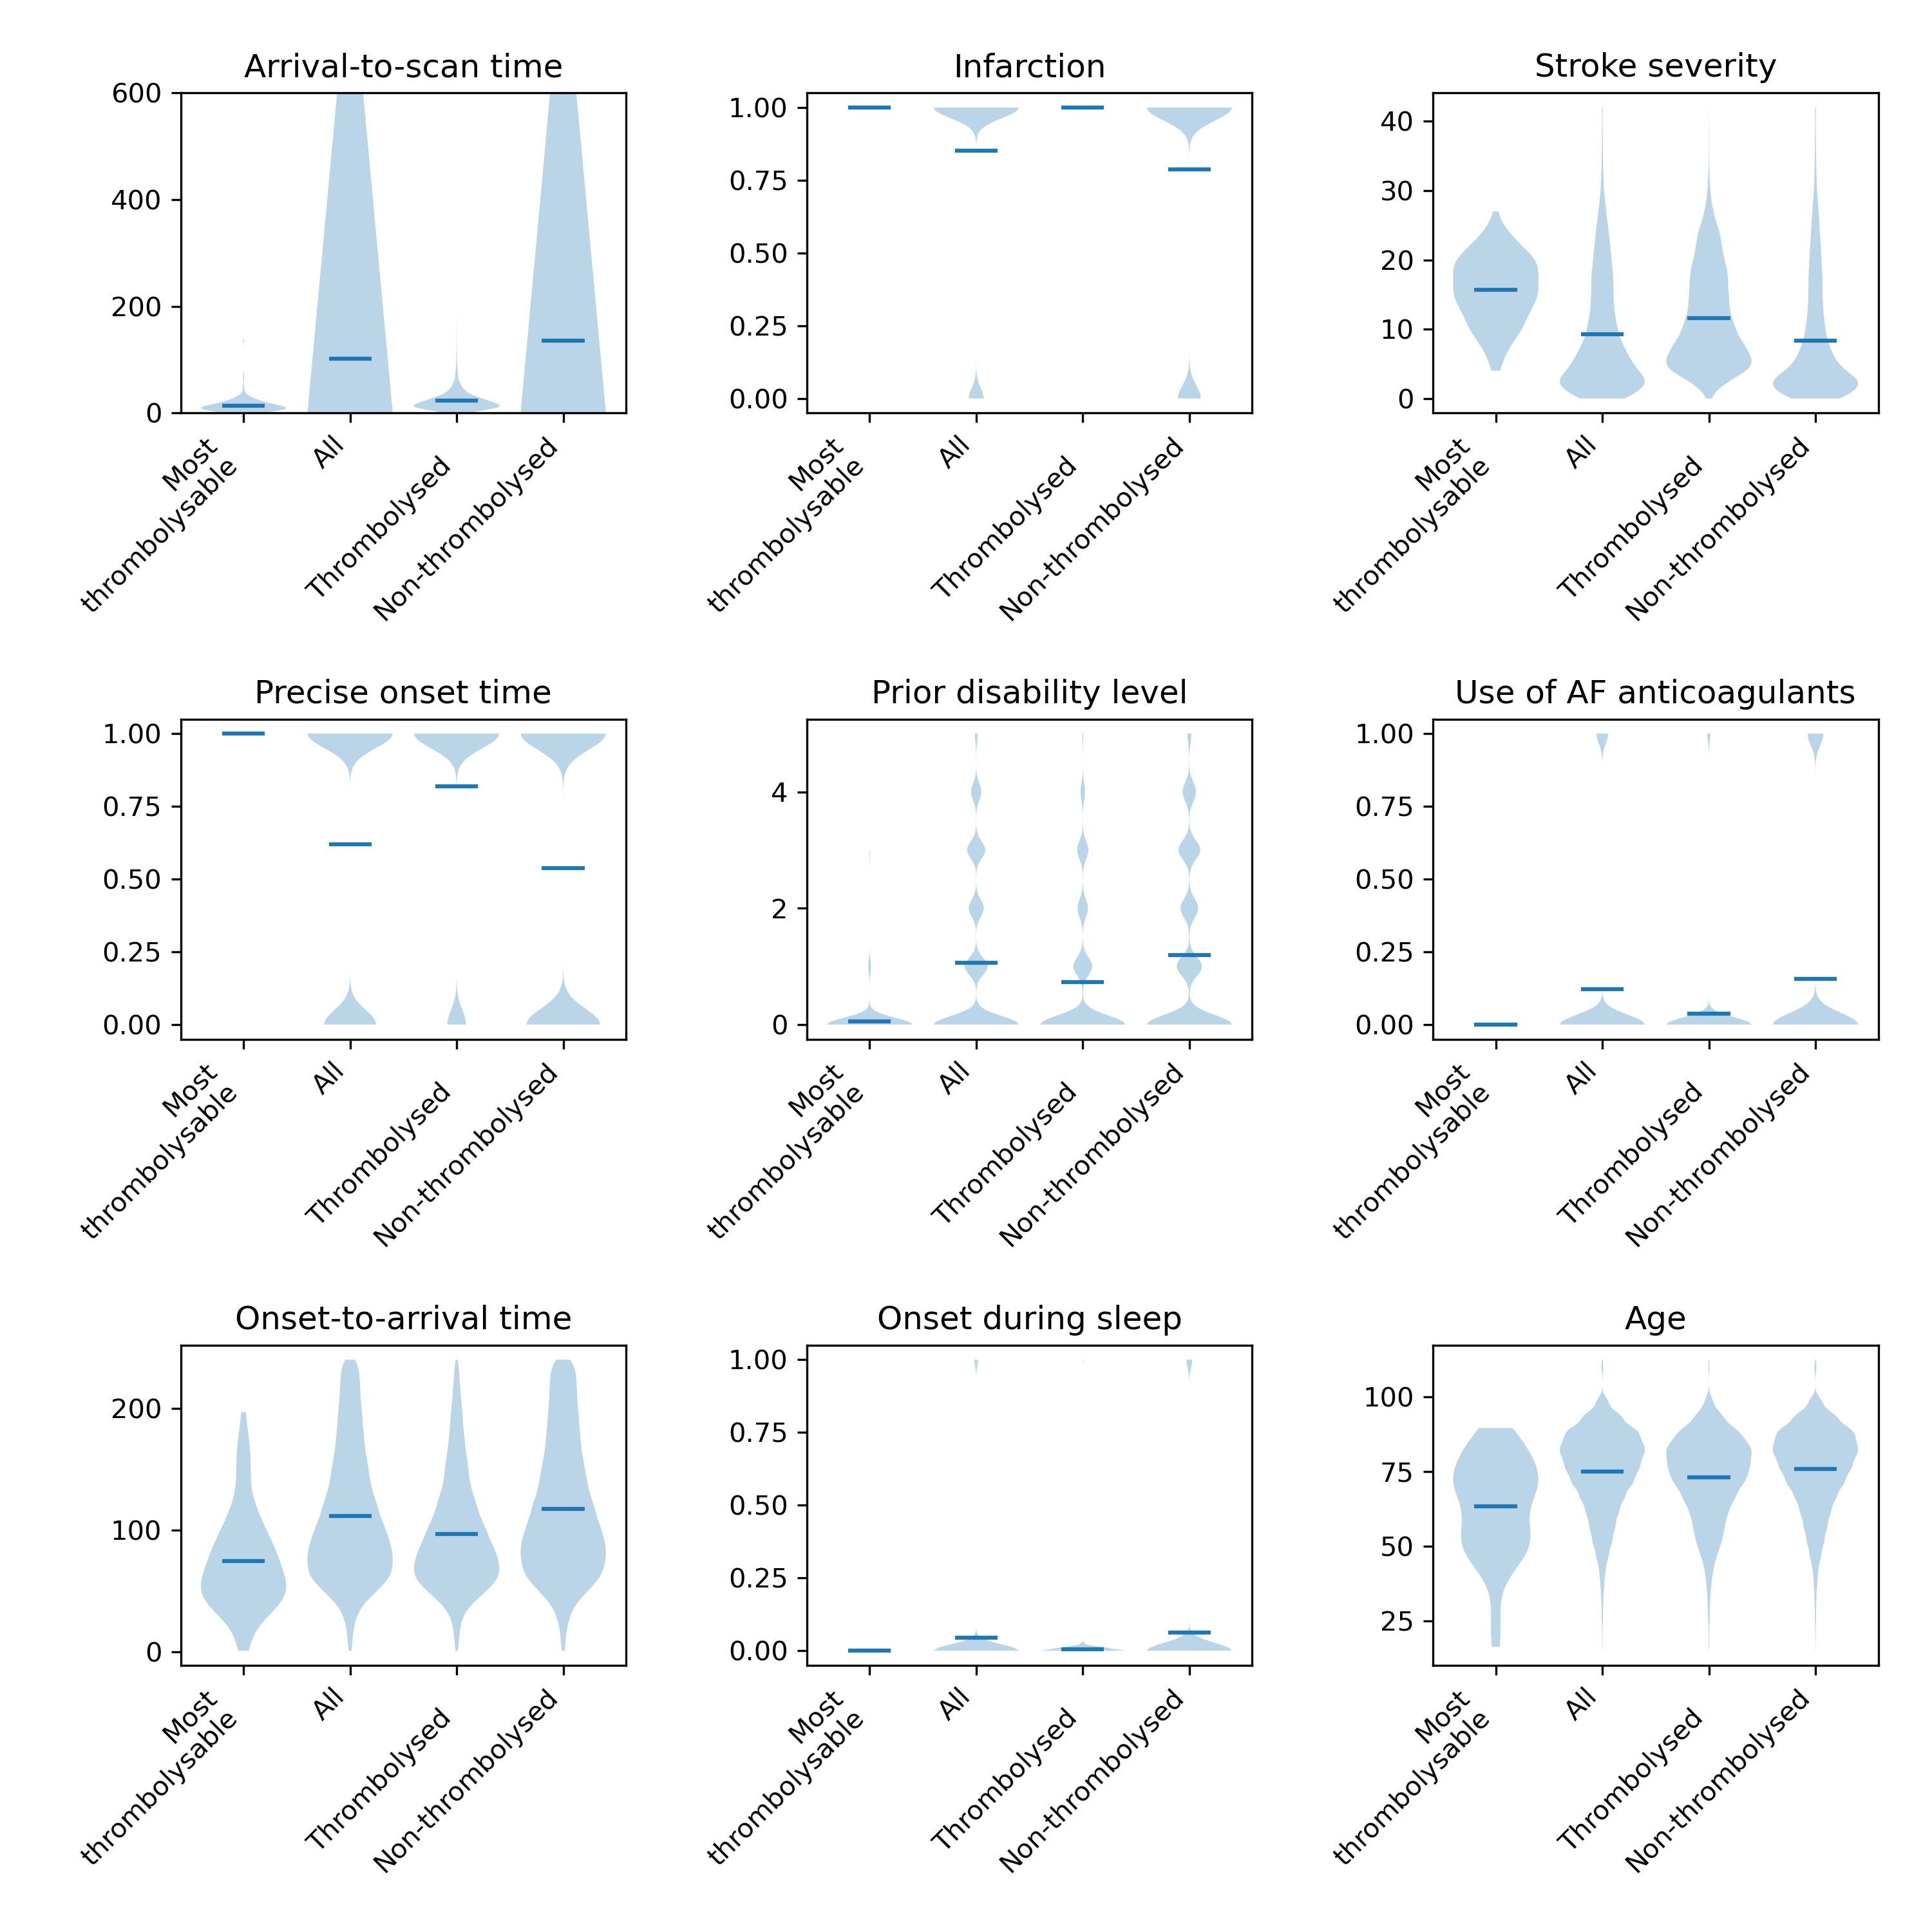
\includegraphics[width=1.0\textwidth]{./images/02a_most_thrombolsyable_violin}
\caption{Violin plots comparing feature values between the patient with the highest probability of thrombolysis at each hospital with all patients, all patients who had received thrombolysis, and all patients who had not received thrombolysis. Horizontal lines show the mean value of each group.}
\label{fig:results_most_thrombolysable}
\end{figure}

%%%%%%%%%%%%%%%%%%%%%%%%%%%%%%%%%%%%%%%%%%%%%%%%%%%%%%%%%%%%%%%%%%%%%%%%

\subsection{Waterfall plots of SHAP values}

Waterfall plots show the influence of features for an individual prediction. We generally handle SHAP values as how they affect log odds of receiving thrombolysis, but for individual predictions, probability plots are more intuitive. Figure \ref{fig:results_waterfall} shows an example of a patient with low (top) and high (bottom) probability of receiving thrombolysis. The model starts with a base prediction of a 24\% probability of receiving thrombolysis, before feature values are taken into account. For the patient with a low probability of receiving thrombolysis, the two most influential features reducing the probability of receiving thrombolysis are a long arrival-to-scan time (138 minutes) and a low stroke severity (NIHSS=2). For the patient with a high probability of receiving thrombolysis, the two most influential features increading the probability of receiving thrombolysis are a short arrival-to-scan time (17 minutes) and a moderate stroke severity (NIHSS=14). 

\begin{figure}
\centering
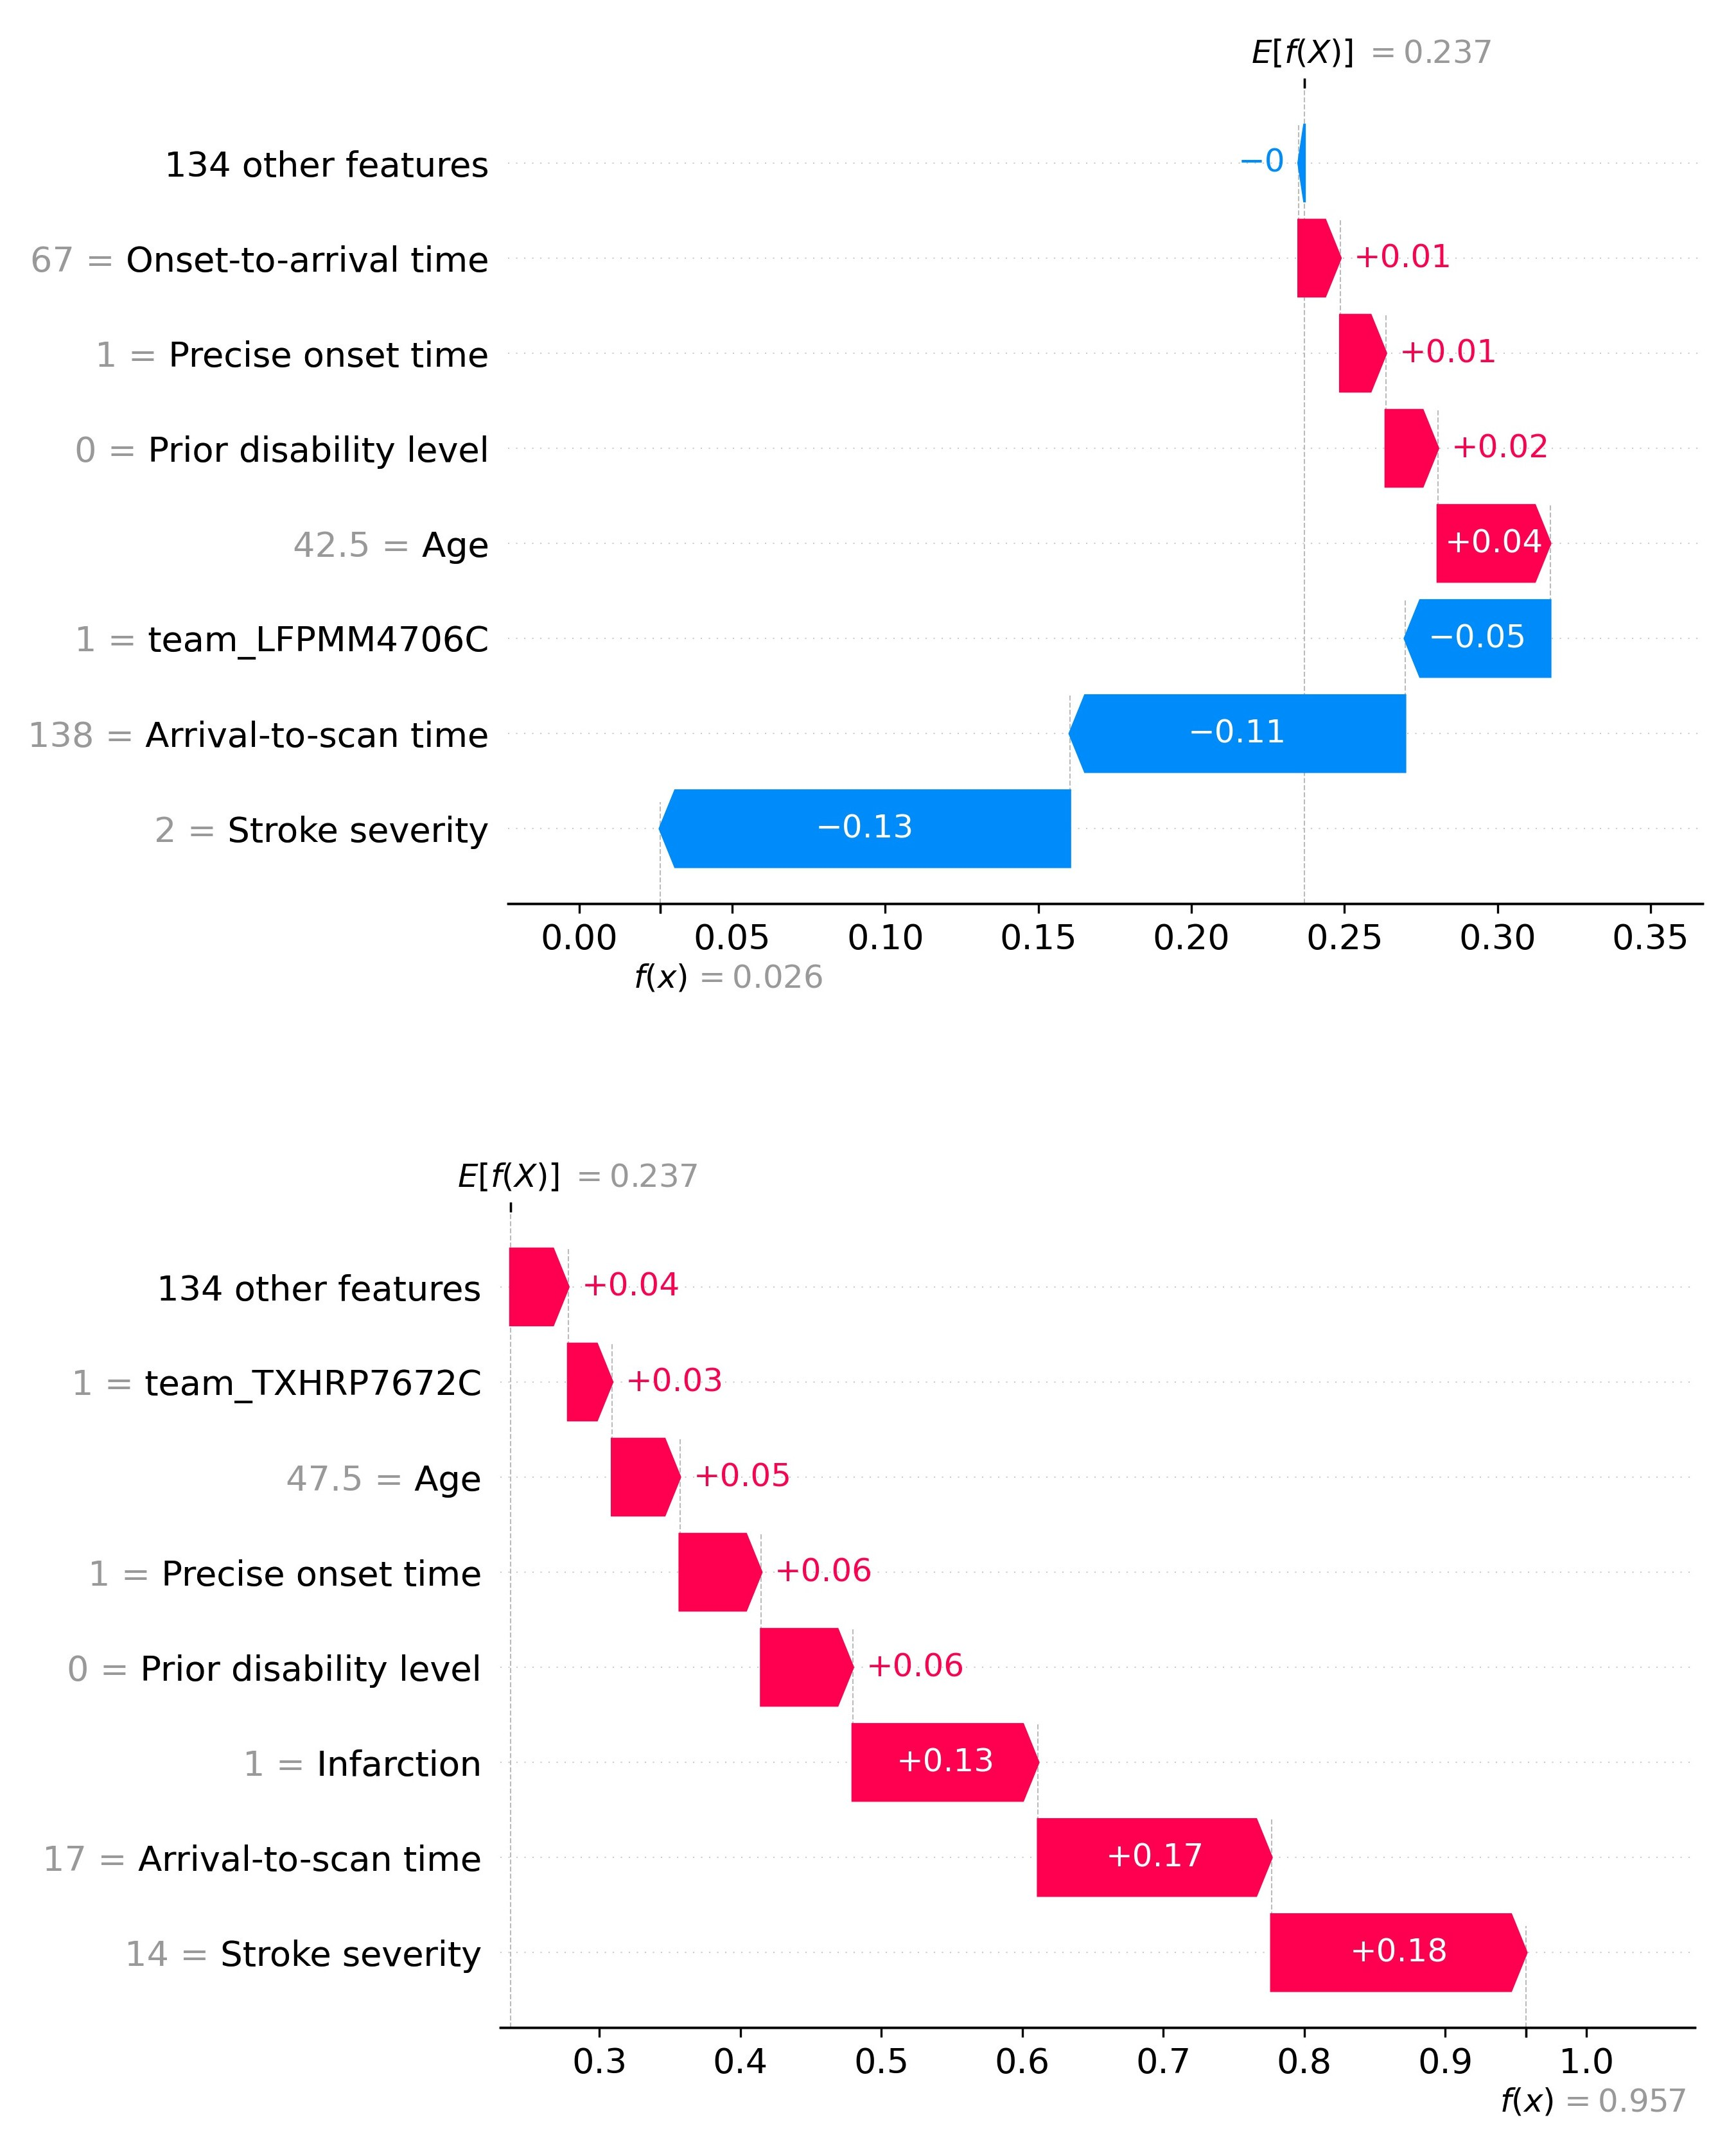
\includegraphics[width=0.8\textwidth]{./images/waterfall}
\caption{Waterfall plots showing the influence of each feature on the predicted probability of a single patient receiving thrombolysis. Top: An example of a patient with a low probability (2.6\%) of receiving thrombolysis. Bottom: An example of a patient with a high probability (95.7\%) of receiving thrombolysis.}
\label{fig:results_waterfall}
\end{figure}

\subsection{The relationship between feature values and the odds of receiving thrombolysis}

SHAP values provide the influence of each feature, as the change in log-odds of receiving thrombolysis. SHAP values expressed as log-odds are additive, that is the final log-odds of receiving thrombolysis is the sum of the base model prediction (the log-odds of receiving thrombolysis before feature influences are considered), and the SHAP values for each feature (these include interactions with other features).

Violin plots (figure \ref{fig:results_shap_violin} show the relationship between feature values and SHAP values for individual patients. Key observations are, with SHAP influence converted to from log-odds to odds:

\begin{itemize}
    \item \emph{Stroke type}: The SHAP values for stroke types effectively eliminated any chance of receiving thrombolysis for non-ischaemic (haemorrhagic) stroke.
    \item \emph{Arrival-to-scan time}: The odds of receiving thrombolysis reduced by about 20 fold over the first 100 minutes of arrival to scan time.
    \item \emph{Stroke severity (NIHSS)}: The odds of receiving thrombolysis was lowest at NIHSS 0, rose and peakws at NIHSS 15-25, and then fell again with higher stroke severity. The difference between minimum odds (at NIHSS 0) and maximum odds (at 15-25) of receiving thrombolysis was 30-35 fold.
    \item \emph{Stroke onset time type (precise vs. estimated)}: The odds of receiving thrombolysis were about 3 fold greater for precise onset time than estimated onset time.
    \item \emph{Disability level (Rankin) before stroke}: The odds of receiving thrombolysis fell about 5 fold between mRS 0 and 5.
\end{itemize}


\begin{figure}
\centering
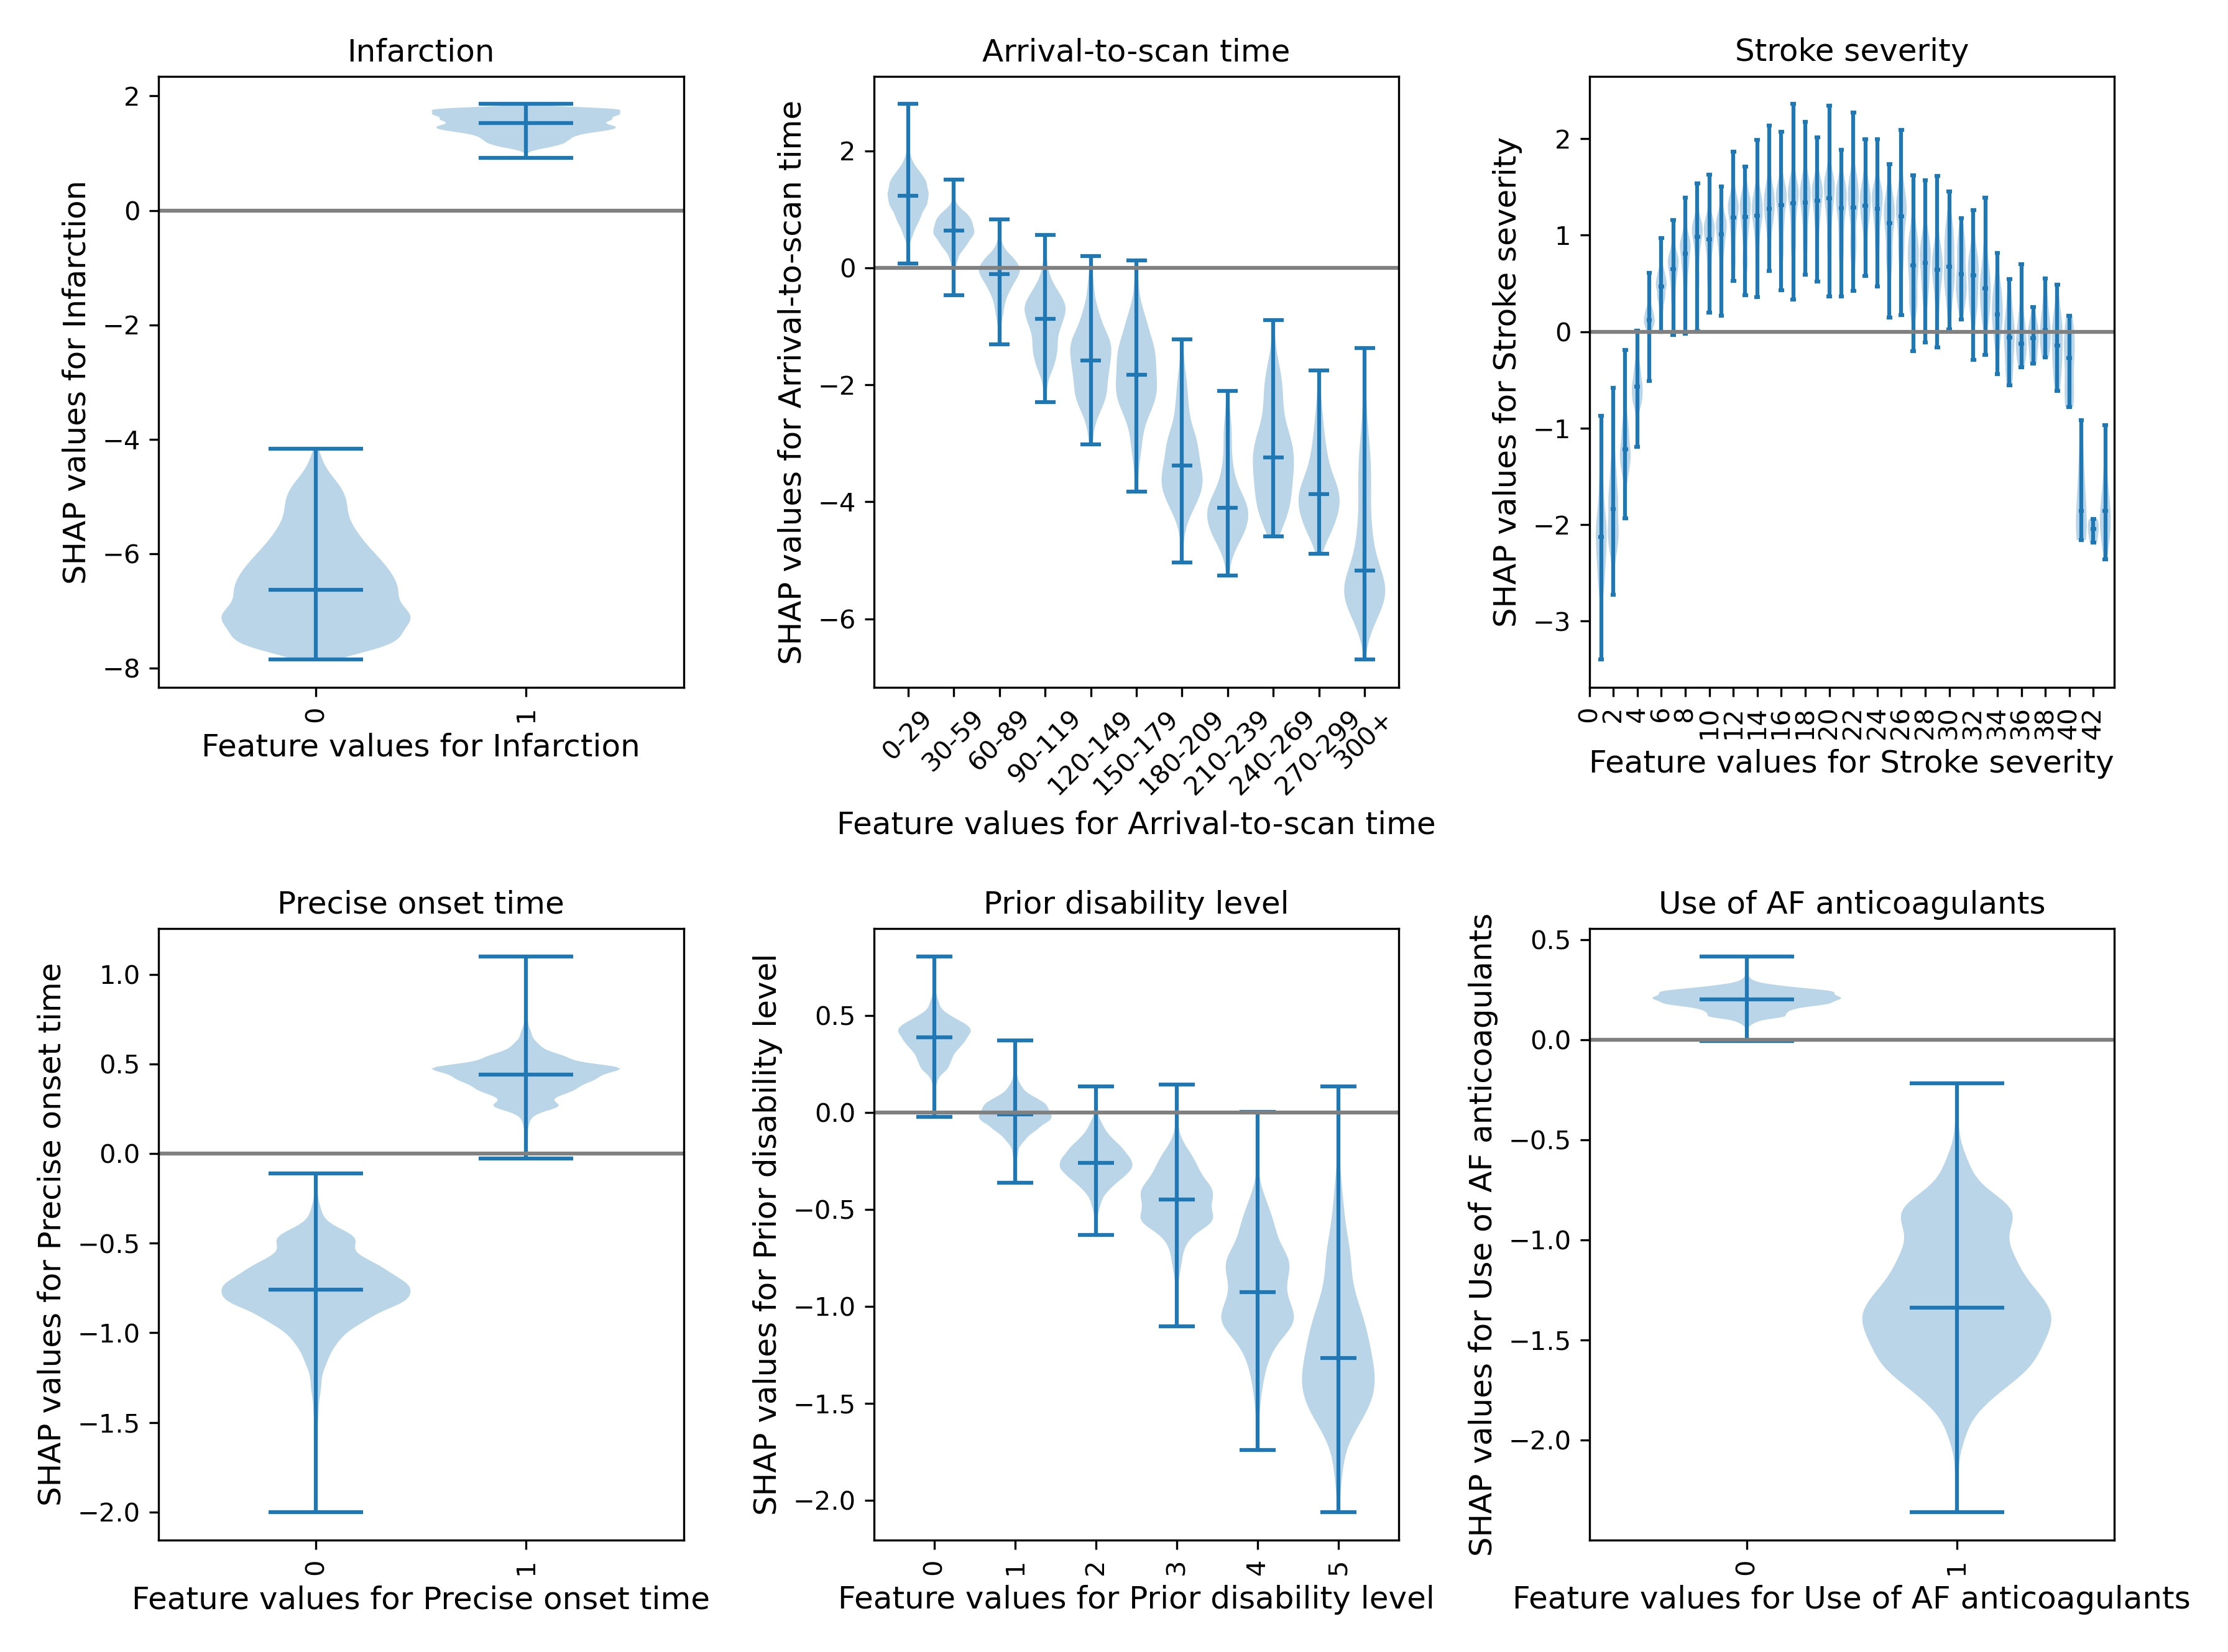
\includegraphics[width=1\textwidth]{./images/03_xgb_10_features_thrombolysis_shap_violin}
\caption{Violin plots showing the relationship between SHAP values and feature values. The horizontal line shows the median SHAP value. SHAP values were taken from the training set of the first of 5 k-fold train/test splits.}
\label{fig:results_shap_violin}
\end{figure}

%%%%%%%%%%%%%%%%%%%%%%%%%%%%%%%%%%%%%%%%%%%%%%%%%%%%%%%%%%%%%%%%%%%%%%%%

\subsection{Hospital SHAP values and predicted use of thrombolysis in a 10k cohort of patients}

When examining SHAP, we took the hospital SHAP values for patients attending each hospital. When we examined the hospital SHAP values only for patients attending each hospital, the hospital SHAP values ranged from -1.4 to +1.4. This range of SHAP (log odds) represents a 15 fold difference in odds of receiving thrombolysis between hopsitals (most are in the range of -1 to +1, but this still represents a 7-8 fold difference in odds of receiving thrombolysis).

We compared the hospital SHAP value with the observed thrombolysis use at each hospital. Hospital SHAP correlated with observed thrombolysis rate with an r-squared of 0.582, suggesting that 58\% (P<0.0001) of the between-hospital variance in thrombolysis use may be explained by the hospitals' SHAP values, that is the hospitals' predisposition to use thrombolysis.

We used a 10k cohort of patients (not used in training the model) to predict between-hospital differences in use of thrombolysis if all hospitals had the same patients arriving. All patient feature values were kept constant, except the hospital coding was changed to mimic all patients attending each of the 132 hospitals. Predicted use of thrombolysis in the same 10k cohort ranged from 10\% to 45\%. We found that the median hospital SHAP value for the 10k patients correlated very closely with the predicted thrombolysis use in the 10k cohort at each hospital (r-squared = 0.947), confirming that the hospital SHAP is providing a direct insight into a hospital's propensity to use thrombolysis.


%%%%%%%%%%%%%%%%%%%%%%%%%%%%%%%%%%%%%%%%%%%%%%%%%%%%%%%%%%%%%%%%%%%%%%%%

\subsection{How individual hospitals may modify general patterns of thrombolysis}

SHAP values are composed of a \emph{main effect} of a feature, and \emph{interaction effects} with other features. The main effect captures the general pattern use of thrombolysis across hospitals independent of other feature values, and independent of which hospital a patient attended. The interaction may either strengthen or attenuate the main effect. For example the main effect of knowing a stroke onset time precisely is to increase the odds of receiving thrombolysis, as indicated by a positive SHAP values. Individual hospitals, in addition to having a general effect of influencing the odds of receiving thrombolysis, may selectively adjust the influence of other features such knowing the stroke onset time precisely, with some teams strengthening the effect, leading to a larger difference in odds of receiving thrombolysis depending on whether stroke onset time is known precisely, whereas other teams will attenuate the main effect, leading to a smaller difference in odds of receiving thrombolysis.

Figure \ref{fig:results_shap_hosp_intercations} shows examples of hospitals which either attenuated or strengthened the main effect of whether a stroke onset time is known precisely, the effect of stroke severity, or the effect of pre-stroke disability. These SHAP interactions revealed how individual hospitals may differ in the influence of specific patient features.

\begin{figure}
\centering
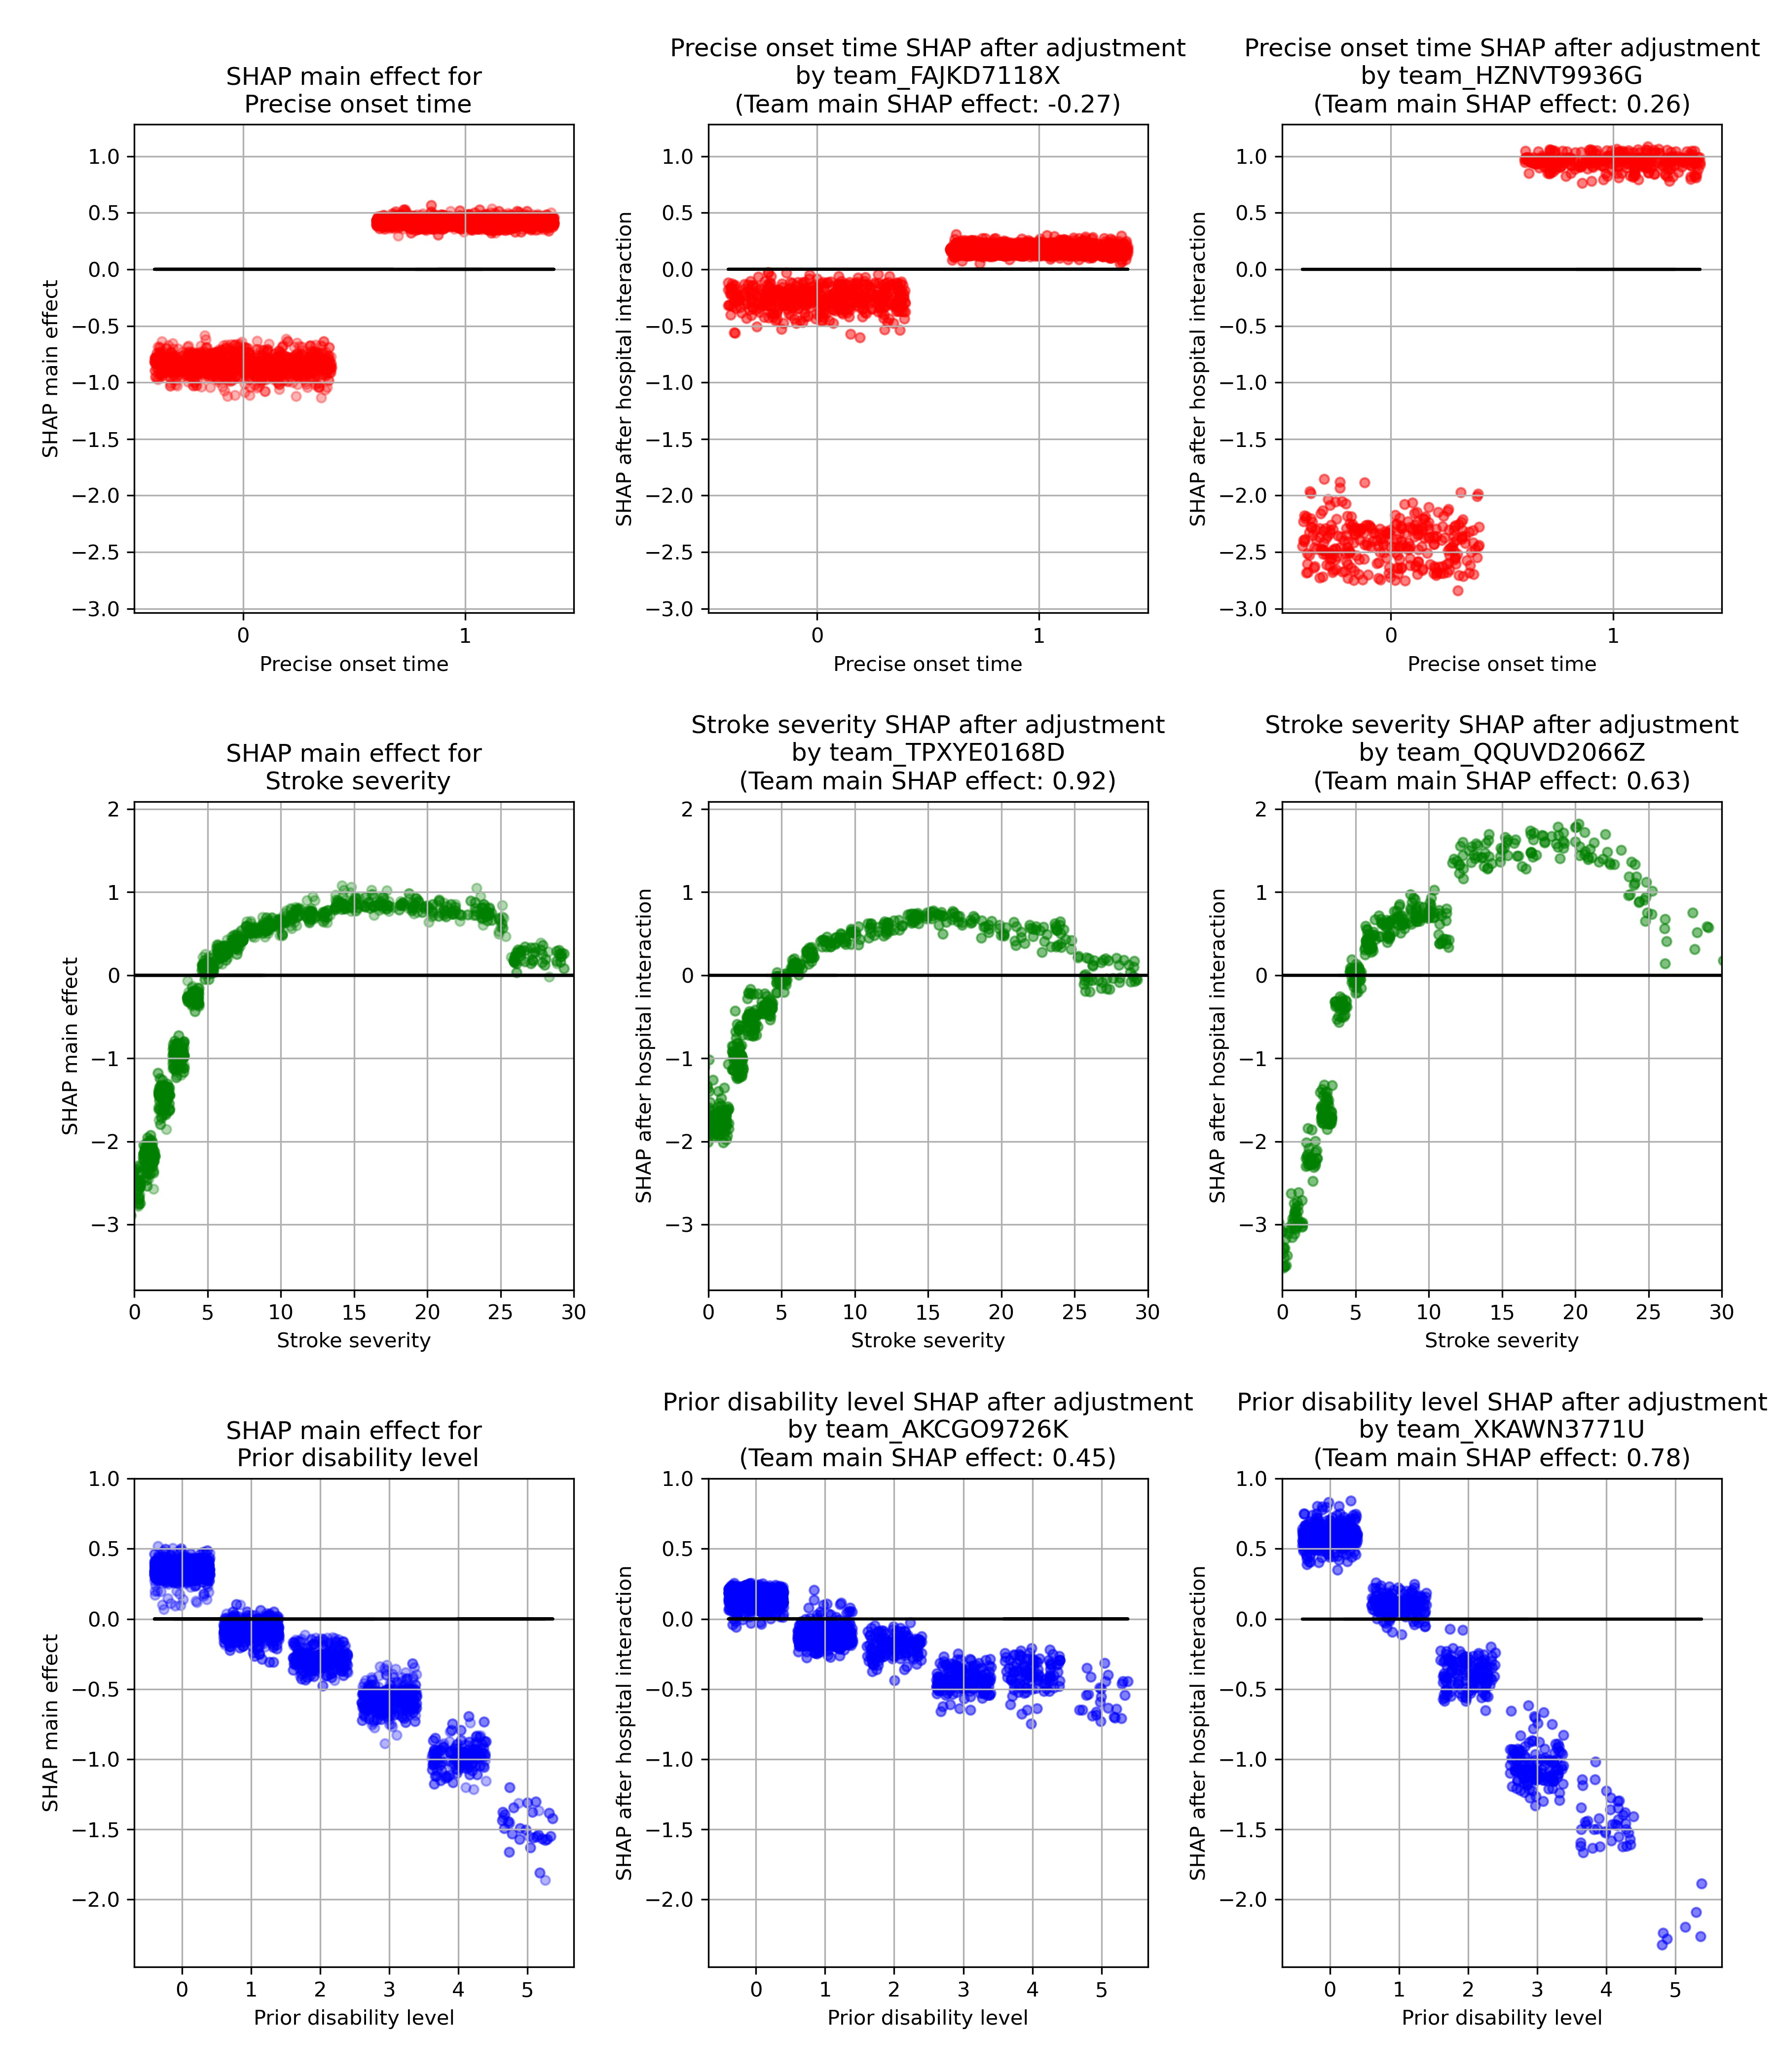
\includegraphics[width=1.0\textwidth]{./images/12aa_three_way_shap_adjustment}
\caption{Adjustment of SHAP main effects by individual hospital. Each row first (left) shows the main SHAP effect of the feature, then (middle) a hospital where the SHAP interaction attenuates the main effect, and finally (right) a hospital where the SHAP interaction strengthens the main effect. Top row (red): main SHAP effect and adjusted SHAP values for precise stroke onset time. Middle row (green): main SHAP effect and adjusted SHAP values for stroke severity. Bottom row (blue): main SHAP effect and adjusted SHAP values for pre-stroke disability.}
\label{fig:results_shap_hosp_intercations}
\end{figure}

%%%%%%%%%%%%%%%%%%%%%%%%%%%%%%%%%%%%%%%%%%%%%%%%%%%%%%%%%%%%%%%%%%%%%%%%

\subsection{Subgroup analysis}

We analysed the observed and predicted use of thrombolysis in subgroups of patients. Those groups were:

\begin{itemize}
  \item An 'ideal' thrombolysable patient:
  \begin{itemize}
    \item Stroke severity NIHSS in range 10-25
    \item Arrival-to-scan time $<$30 minutes
    \item Stroke type = infarction
    \item Precise onset time = True
    \item Prior disability level (mRS) = 0
    \item AF anticoagulants = False
    \item Onset-to-arrival time $<$90 minutes
    \item Age $<$80 years
    \item Onset during sleep = False
  \end{itemize}
  \item Mild stroke severity (NIHSS $<$5)
  \item No precise onset time
  \item Existing pre-stroke disability (mRS $>$2)
\end{itemize}

For the observed thrombolysis use, data was limited to the patients attending each hospital (and so the patient mix was different for each hospital). For the predicted thrombolysis use the predictions were based on the 10k patient cohort for all hospitals.

Figure \ref{fig:results_boxplot} shows a boxplot of either observed and predicted use of thrombolysis, broken down by subgroup. The three subgroups of NIHSS $<$5, no precise stroke onset time, and pre-stroke mRS $>2$, all had reduced thrombolysis use, and combining these non-ideal features reduced thrombolysis use further. The observed and predicted thrombolysis use show the same general patterns, but some small differences existed: 1) The use of thrombolysis in *ideal* patients is a little low in the observed vs actual results (mean hospital thrombolysis use = 89\% vs 99\%), 2) The predicted results show a stronger effect of combining non-ideal features, 3) The observed thrombolysis rate shows higher between-hospital variation than the predicted thrombolysis rate. This may be partly explained by the observed thrombolysis rate being on different patients at each hospital, but may also be partly explained by actual use of thrombolysis being slightly more variable than predicted thrombolysis use (which will follow general hospital patterns, and will not include, for example, between-clinician variation at each hospital).

For both the predicted and observed thrombolysis, subgroup thrombolysis use tended to reduce in parallel (r-squared 0.221 - 0.308 in observed thrombolysis use, and 0.445 to 0.621 in the predicted thrombolysis use).

\begin{figure}
\centering
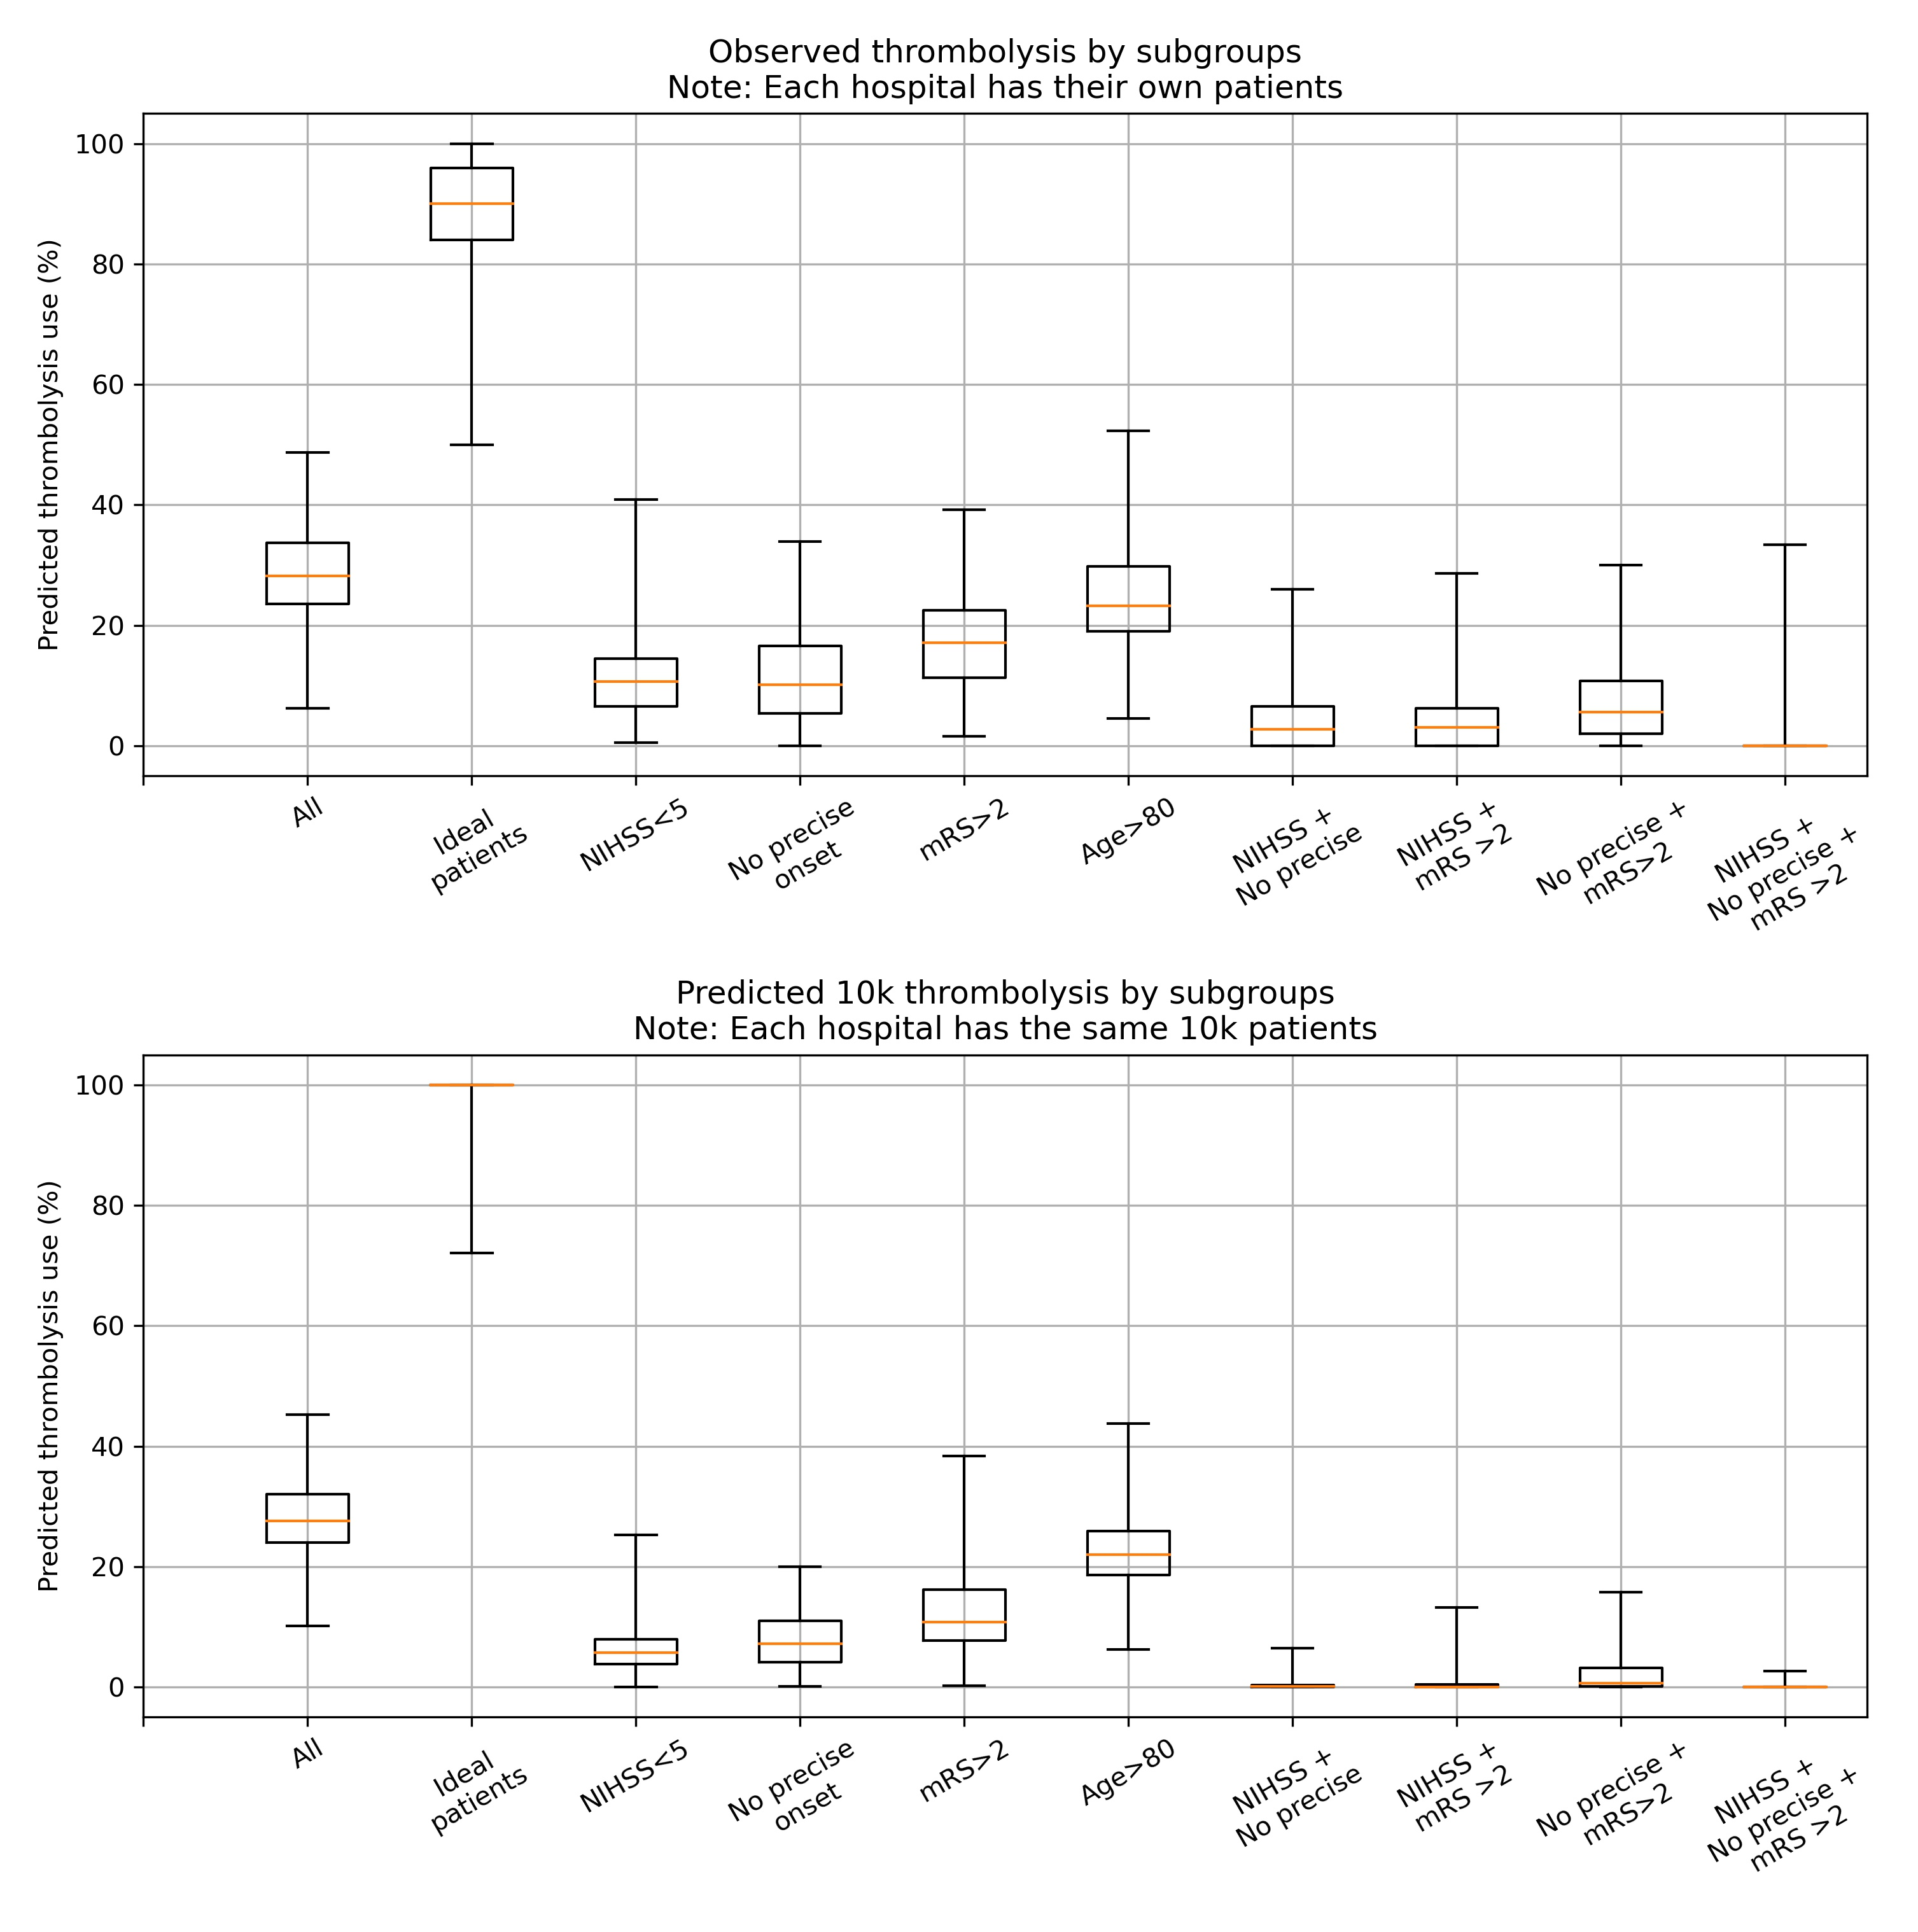
\includegraphics[width=1\textwidth]{./images/15a_actual_vs_modelled_subgroup_violin}
\caption{Boxplot for either observed (top) or predicted (bottom) use of thrombolysis for subgroups of patients.}
\label{fig:results_boxplot}
\end{figure}

%%%%%%%%%%%%%%%%%%%%%%%%%%%%%%%%%%%%%%%%%%%%%%%%%%%%%%%%%%%%%%%%%%%%%%%%%%%%%%%%%%%%%%%%%%%%%

\subsection{Comparing predicted thrombolysis decisions across hospitals, using artificial patients}

Artificial patients may be used to explore how decisions vary between hospitals. For example, a patient with moderate/severe stroke severity (NIHSS=15), infarction, having a precise onset time (and not during sleep), onset-to-arrival of 60 minutes, arrival to scan of 15 minutes, no prior disability, aged 72, and not using anticoagulants for atrial fibrillation, was predictde to receive thrombolysis at all hospitals. But if we took exactly that same patient but changed stroke severity to 5, with the patient also having a non-precise onset time, that patient would be expected to receive thrombolysis in only 35\% of hospitals, with a clear divide between the benchmark hospitals (90\% predicted to give thrombolysis) and non-benchmark hospitals (19\% predicted to give thrombolysis). Figure \ref{fig:results_artifical_shap_waterfall_with_violin} shows SHAP  plots for this patient attending each of 132 hospitals.

\begin{figure}
\centering
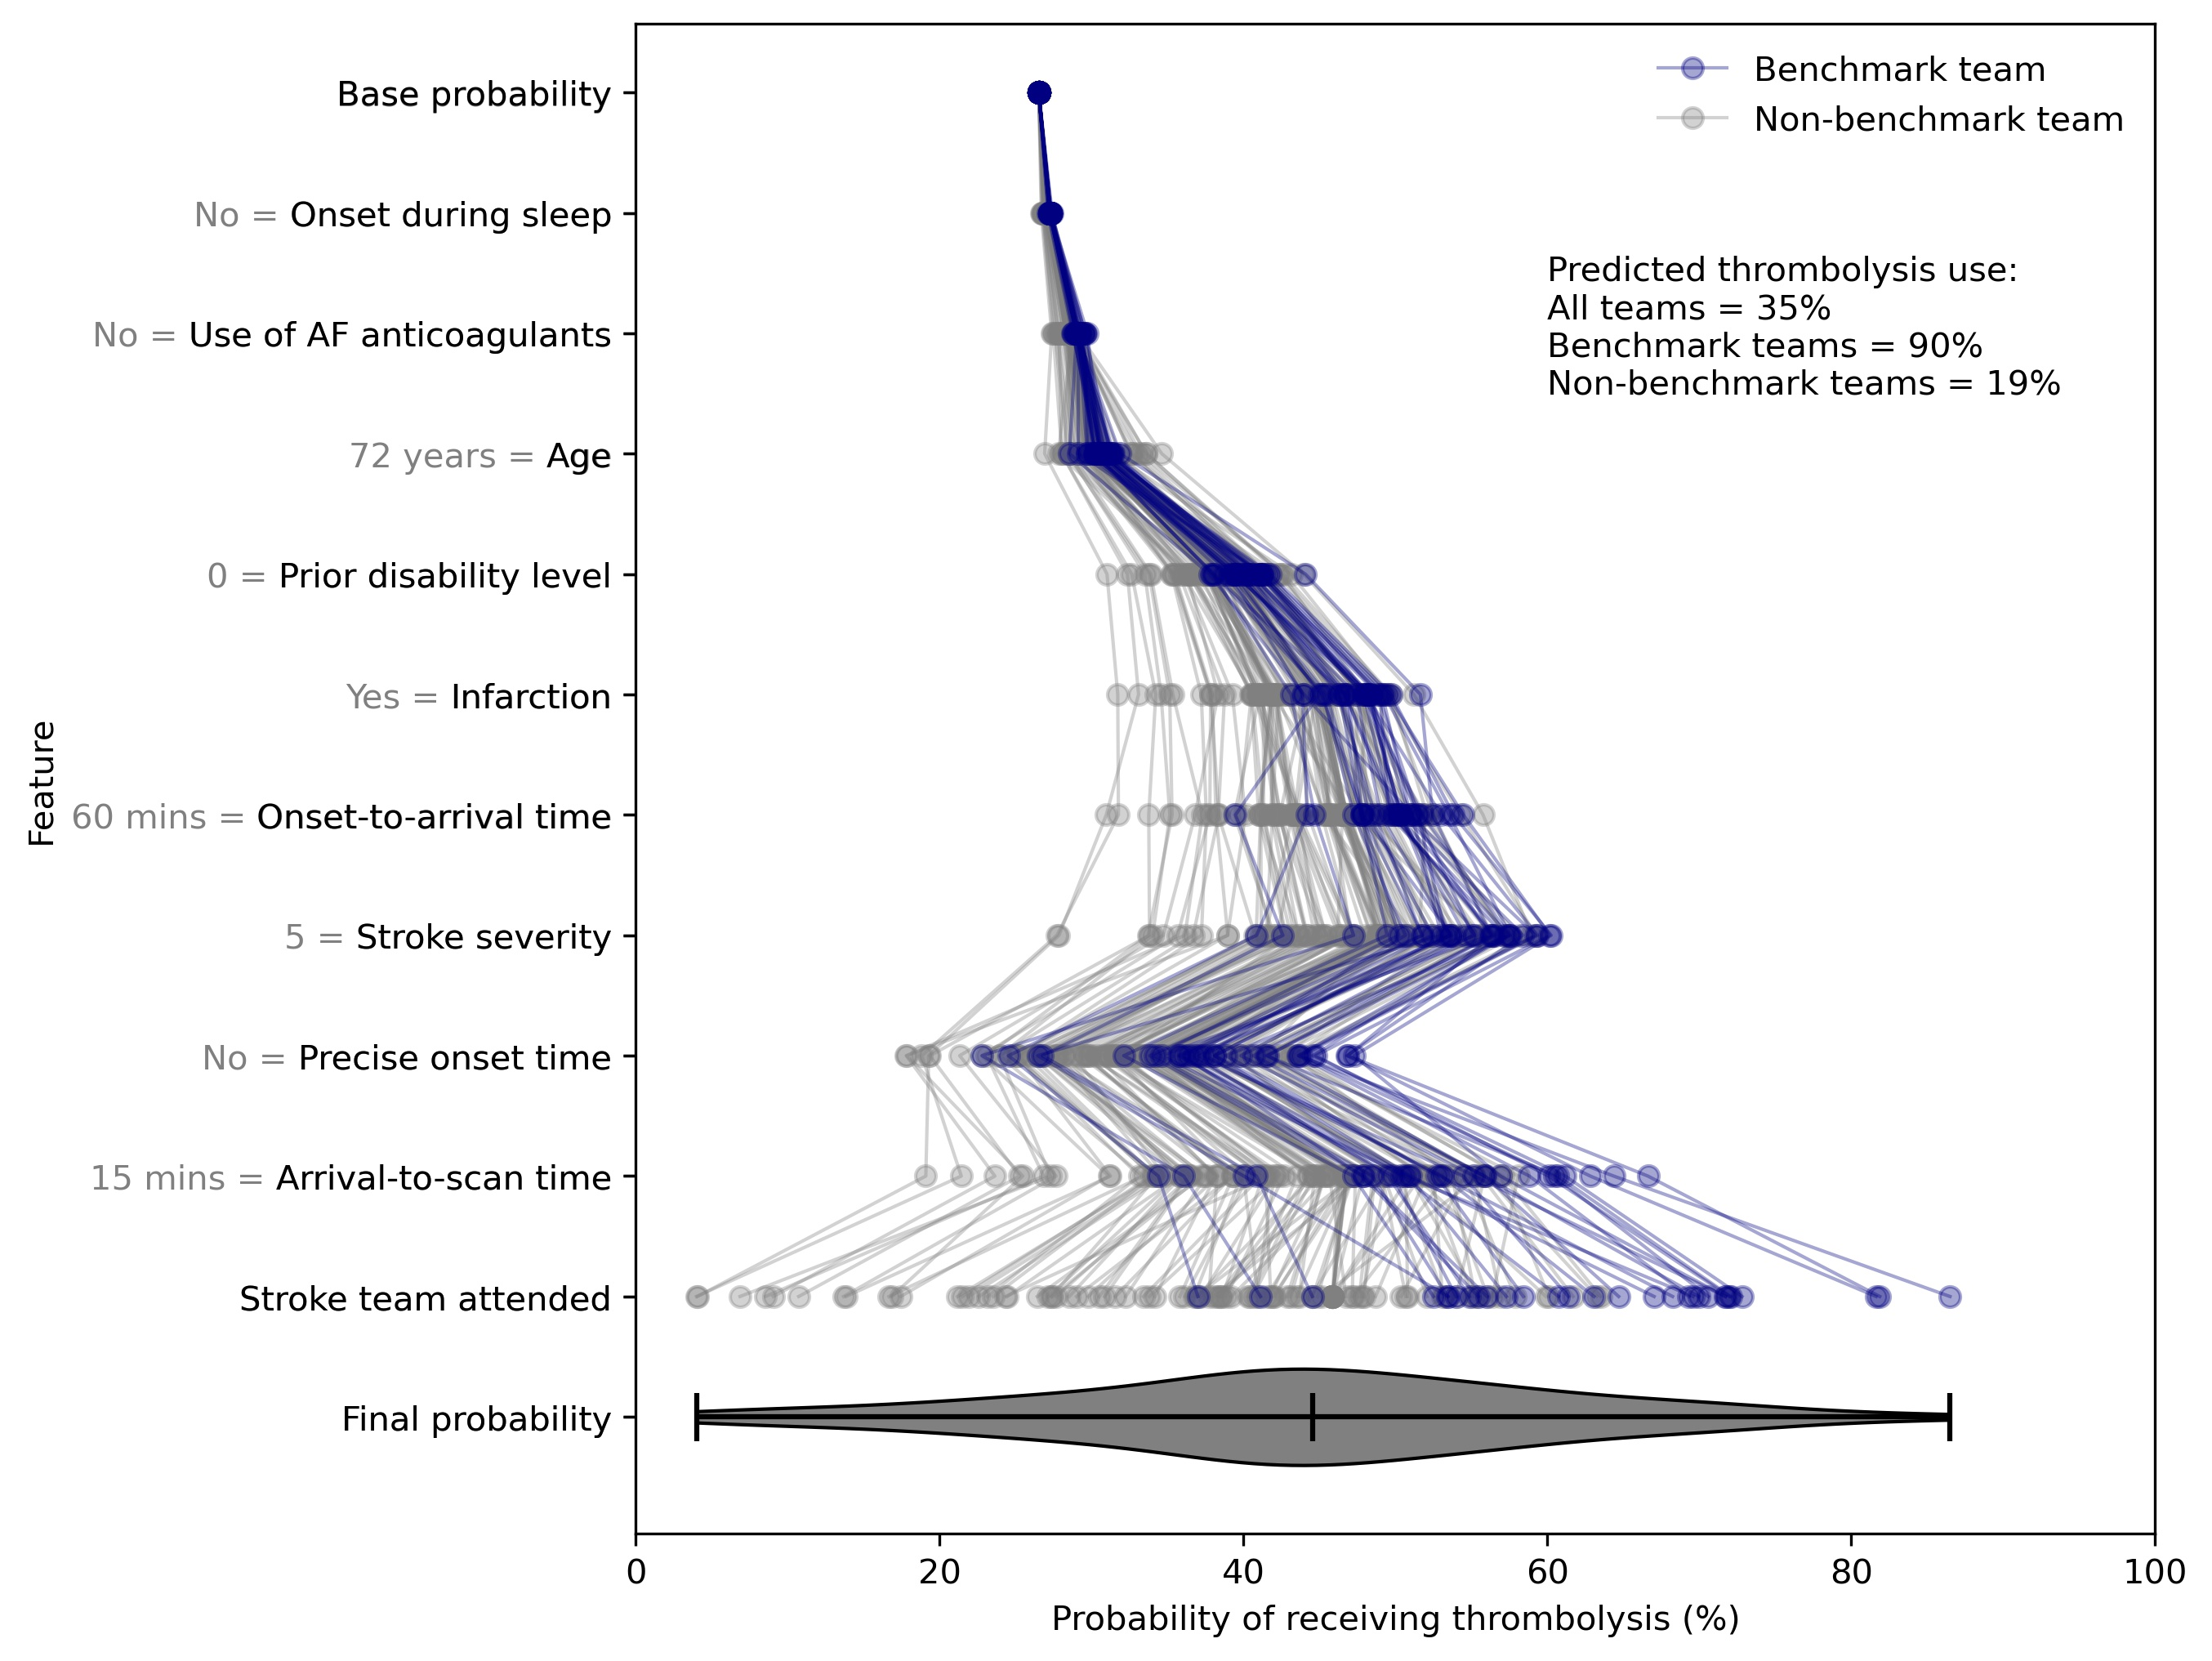
\includegraphics[width=0.85\textwidth]{./images/21_shap_waterfall_with_violin_contentious}
\caption{SHAP plots for the same patient attending 132 different hospitals. The patient has the following feature values: Onset to arrival = 60 mins, Arrival to scan = 15 mins, Infarction = 1, NIHSS = 5, Prior disability level = 0, Precise onset time = 0, Use of AF anticoagulants = 0. The plot shows how each patient feature value contributes to the final prediction of whether that patients is likely to receive thrombolysis. Hospitals coloured blue are \emph{benchmark} hospitals - the 30 hospitals with the highest predicted use of thrombolysis if all hospitals saw the same 10k patient cohort.}
\label{fig:results_artifical_shap_waterfall_with_violin}
\end{figure}








